\chapter{Code Generating AIs}

Code generating AI tools are probably the most prominent application of machine learning in today's software development. They are a category of AI-based development tools which aim at assist developers by automatically producing code-based on the contextual information. Their constant raise in working environments has raised concerns about their potential impact on the software's productivity and quality.

Even though, these tools can help accelerating development and reduce mundane tasks, they also bring forward challenges regarding  maintainability and security. AI generated code could contain small logical error or even vulnerabilities difficult to recognize without human verification. This is why knowing what they can and can't do is essential when introducing them in software development.

This chapter's purpose is to provide an overview of code generating AIs, such as GitHub Copilot, Claude and Cursor. We'll analyze how these tools operate, how they are used in practice ,and the impact they have on software quality and reliability.

\newpage

\begin{table}[h]
\small
\centering
\caption{Feature-based comparison of selected Code Generating AIs}
\resizebox{1\textwidth}{41pt}{
\begin{tabular}{|c|c|c|c|}
\hline
\textbf{Feature} & \textbf{GitHub Copilot} & \textbf{Cursor} & \textbf{Claude}\\
\hline
\textbf{Primary purpose} & Inline code completion \& suggestions & Project-wide code editing \& generation & Large-scale code generation \\
\hline
\textbf{Context awareness} & Limited to opened files & Full project via workspace indexing & Large context window (project-level) \\
\hline
\textbf{IDE integration} & VS Code, JetBrain IDEs, Neovim & Standalone IDE (Based on VS Code) & Web interface / IDE plugins \\
\hline
\textbf{Test generation} & Limited & Prompt-based & Prompt-based \\
\hline
\textbf{User interaction} & Continuous inline suggestions & Command-based & Prompt-based \\
\hline
\textbf{Target audience} & Individual developers & Individual developers \& small teams & Individual developers \\
\hline
\end{tabular}
}
\label{table_3.1}
\end{table}

Table \ref{table_3.1} provides an overview of the main characteristics of the code generating AIs that are considered in this survey, as well as they are used and integrated in the development cycle.

\section{GitHub Copilot}

GitHub Copilot is an AI for code \textit{completion}, released in October 2021, developed by GitHub with the assistance of OpenAI, and it is integrated in various IDEs such as Visual Studio Code, NeoVim, and even JetBrains to mention a few\cite{Copilot}. 

In the beginning Copilot just used OpenAI's GPT\cite{CopilotAPI} but, ever since 2024, it has expanded to include Anthropic's Claude, and even Google's Gemini. According to GitHub, Copilot's main purpose is to help developers get accustomed to new coding frameworks by reducing the time spent reading documentation.

The way that Copilot works is by collecting pre-existing code, written and uploaded onto public GitHub repositories by programmers, and then starts suggesting code snippets which auto-completes our coding when writing it. It can even convert code comments to runnable code and autocomplete repetitive sections, as well as methods and functions.

It is to be noted that even GitHub mentions how Copilot managed to autocomplete correctly roughly half of the times; When given a Python header code it was correct 43\% of the times on it's first attempt and raising to 57\% of the times after ten attempts\cite{CopilotFAQ}.

From a software quality point of view, Copilot could improve the development speed, but it may also introduce hidden errors or reduce the clarity of the code if it is not properly reviewed. As a result, its effectiveness depends on the developer's experience and critical evaluation.

\section{Claude and Claude Code}

Claude is a Large Language Model developed by Anthropic with it's first release being on March of 2023 with Claude 1 and the latest, Claude Opus 4.5, in November of 2025. 

\begin{figure}[H]
    \centering
    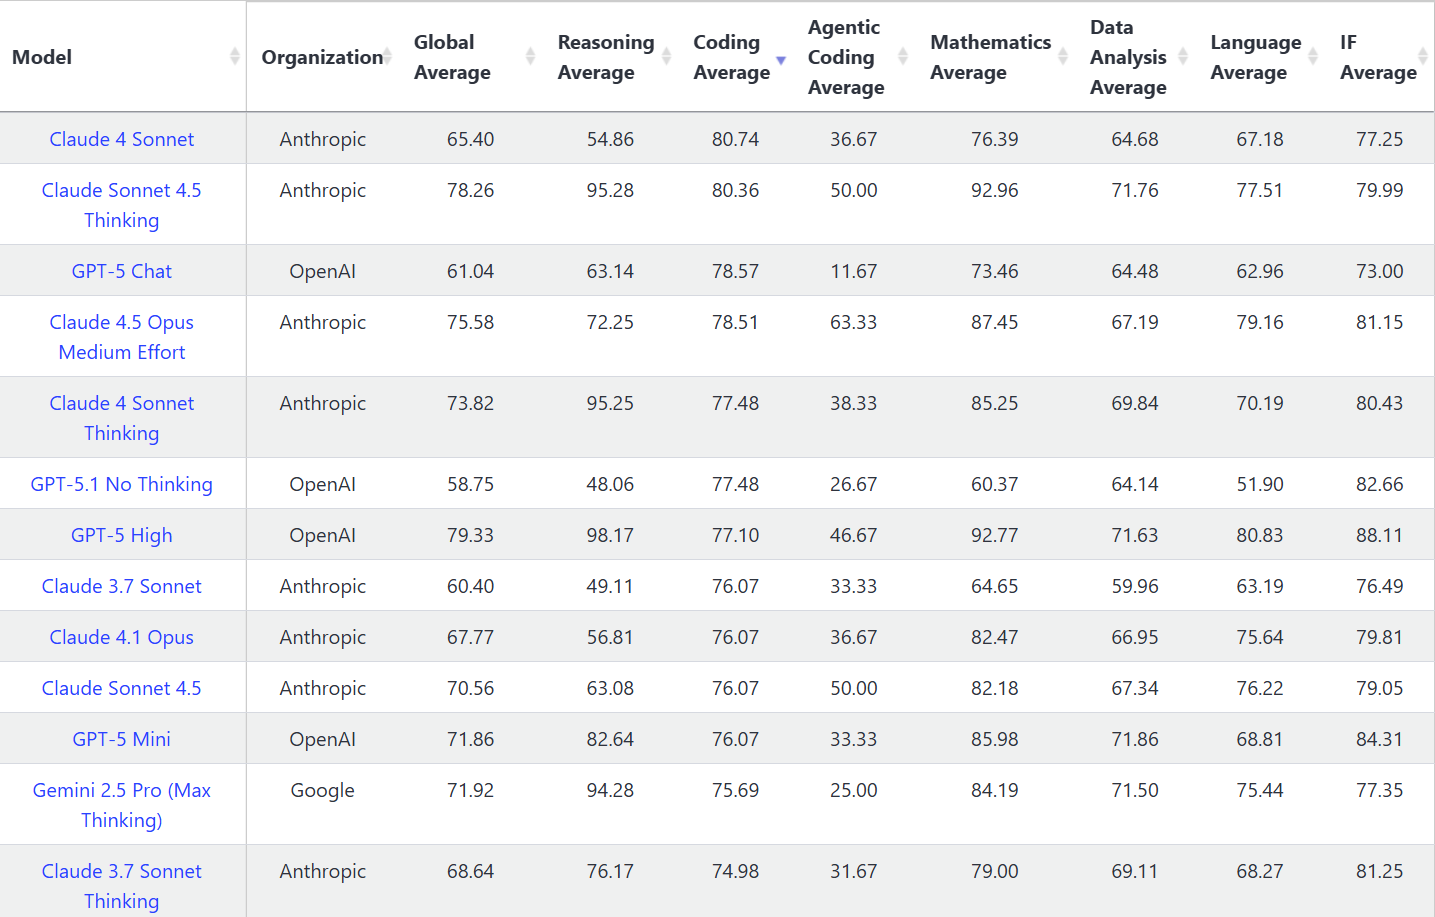
\includegraphics[width=0.95\linewidth]{images/Screenshot 2025-12-23 214938.png}
    \caption{LLMs Benchmark - Coding Average \cite{livebench}}
    \label{fig:AI_Benchmark}
\end{figure}

When Claude first came out coding wasn't one of it's most proficient skills. But now, unlike it's other counterparts, coding has become it's strongest suit, as we can see from this benchmark made for LLMs (filtered by "Coding Average") in which Claude models manage to get the top spots on the leaderboard followed \textit{only} from OpenAI's newest model.

Unlike tools like Cursor and GitHub Copilot, Claude is more often than not accessed through a conventional prompt-based interface, with the possibility to add it to your IDE through plug-ins, which changes the way the tool is used in software engineering. Programmers usually prefer a more traditional interaction, instead of receiving inline suggestions during coding. This type of interaction encourages a deeper reasoning.

Quality wise, Claude has the possibility to help improve code readability by explaining to the programmer what the logic behind given code snippets is. It's important to know that the quality of the output depends almost entirely on the prompt the developer gives, which shows how important human reviewing is when such tools are introduced in software development.

\section{Cursor IDE}

Cursor is an Integrated Development Environment with an LLM embedded in it. It was released in 2023, a little over two years ago, and it just recently had it's first stable release, Cursor 2.0, which came out on October 29th 2025.\cite{CursorRelease}. 

\begin{figure}[H]
    \centering
    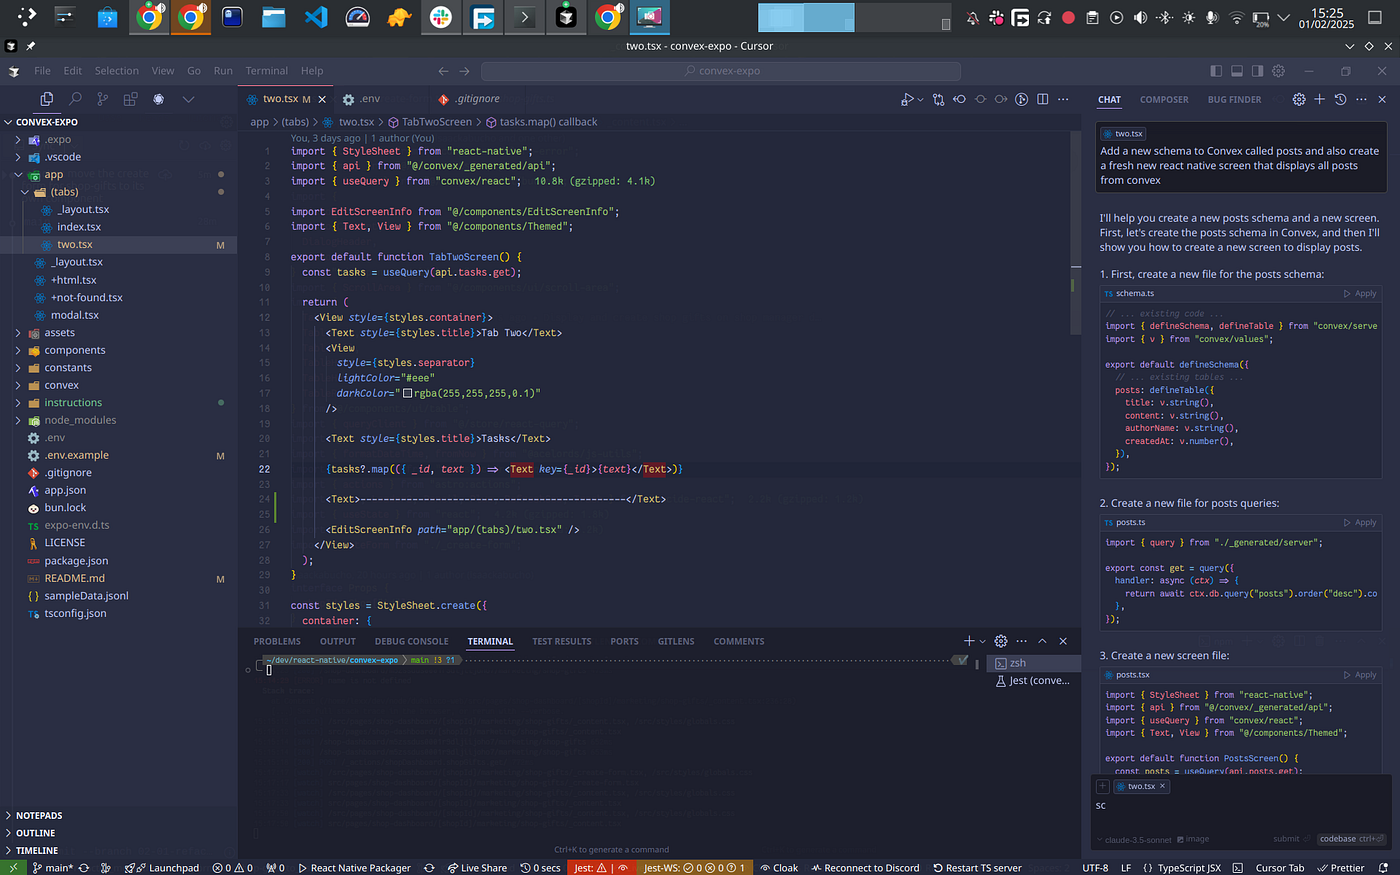
\includegraphics[width=0.95\linewidth]{images/1_P0MD8MiEGvIEdNFZpfkm5Q.png}
    \caption{Cursor IDE GUI \cite{CursorGUI}}
    \label{fig:Cursor_IDE}
\end{figure}

It was made as a fork of the Visual Studio Code IDEs\cite{VSCodeIDE}, and as such the transition from one IDE to the other is smooth and easy, which has made many developers start to switch from VSCode, but also from other unrelated IDEs, to Cursor due to its AI integration and quality of life features such as error detection and automated fixing that the environment offers, as well as the automatic code generation from a user generated prompt.

Of course, such a tool comes with its flaws. As mentioned by Yulia Kumar and her colleagues\cite{kumar2025evaluating}, Cursor can be a double-edged sword: it helps you find the problem and fix it, but it will not explain \textit{why} it does what it does. This means that as programmers we went from not understanding how the code works to not understanding how an error got fixed. They also mentioned that people with no prior coding experience were able to learn the IDE in just four days, code a functioning app in just three weeks, but needed an additional six weeks just to understand what the LLM had written. 